\documentclass[conference]{IEEEtran}
\usepackage[utf8]{inputenc}
\usepackage{amsmath,amssymb,graphicx,booktabs}

\usepackage[hidelinks,unicode,pdftitle={Layer-Group Coefficient Search for Qwen2.5-0.5B Merging: A Null Test of Layer-Group Search},pdfauthor={Dheiver Francisco Santos},pdfkeywords={model merging, layer-wise merging, validation overfitting, winner's curse, Qwen2.5},pdfsubject={Preprint, Figshare, doi:10.6084/m9.figshare.35013997}]{hyperref}
\begin{document}

\title{Layer-Group Coefficient Search for Qwen2.5-0.5B Merging: A Null Test of Layer-Group Search}

\author{\IEEEauthorblockN{Dheiver Francisco Santos, PhD}
\IEEEauthorblockA{Independent Researcher\\
Maceió, Alagoas, Brazil\\
ORCID: https://orcid.org/0000-0002-8599-9436\\
Preprint, Figshare, 2026, \href{https://doi.org/10.6084/m9.figshare.35013997}{doi:10.6084/m9.figshare.35013997}, CC BY 4.0}}

\maketitle

\begin{abstract}
Interpolating Qwen2.5-0.5B and Qwen2.5-0.5B-Instruct with one global coefficient $t$ leaves open whether per-layer coefficients help. We pre-registered that a coordinate search over four layer groups would beat the global $t^*$ on validation, with a smaller advantage on test (the winner's curse). The search used 21 validation evaluations (1{,}199 items from four benchmarks) and 3{,}967 disjoint test items. The validation gain over $t^*=0.7$ is $+0.83$ pp, within noise (paired 95\% CI $[-0.58,+2.17]$). On test the gain is $+0.39$ pp [$-0.38$, $+1.15$], $p=0.311$, not distinguishable from zero (no equivalence test); this is the primary comparison, as worded in hypothesis 5. Against the best original model (base, 0.5025) the layer-wise merge scores 0.5129, a gain of $+1.04$ pp [$+0.20$, $+1.93$] with nominal $p=0.017$. The pre-registered general rule (paired CI above zero) is met nominally, and fails only the Bonferroni threshold of 0.0083, added later, so we do not claim an improvement. The data are consistent with both a winner's curse and no shrinkage. Scope: one model pair, four benchmarks, one search run.
\end{abstract}

\begin{IEEEkeywords}
model merging, layer-wise merging, validation overfitting, winner's curse, Qwen2.5
\end{IEEEkeywords}

\section{Introduction}
Linear interpolation of a base and an instruction-tuned model has one knob, the coefficient $t$. Because networks are not uniform, it is tempting to give each layer its own coefficient and search for the best combination. More knobs mean more candidates scored on the same validation items, and the best-scoring candidate is partly selected for its noise. This article measures how much of the validation gain of a small layer-wise search survives on items never used for selection.

The setting is deliberately small. Qwen2.5-0.5B and Qwen2.5-0.5B-Instruct \cite{yang2024qwen25} share architecture and tokenizer. A single-$t$ grid over $\{0,0.1,\dots,1\}$ gave a validation-selected $t^*=0.7$. The question, pre-registered as hypothesis 5, is whether searching four layer groups from $t^*$ improves on $t^*$ on validation, and whether that improvement carries to test. The primary comparison is the layer-wise merge against the global $t^*$; the comparison against the best original is secondary. We find a validation gain within validation noise and a test gain over $t^*$ not distinguishable from zero (no equivalence test). The test gain over the best original is nominally significant but fails multiplicity correction.

\section{Related Work}
\textbf{Layer-wise coefficients.} AdaMerging learns task-wise or layer-wise merging coefficients without labeled data, by minimising prediction entropy on unlabeled samples \cite{yang2023adamerging}. LoraHub composes LoRA modules with coefficients found by gradient-free optimization on a few examples \cite{huang2023lorahub}. Interpolation coefficients are conventionally chosen on held-out data in weight-space ensembling and in task arithmetic \cite{wortsman2022wise,ilharco2022editing,wortsman2022soups}, and MergeKit exposes per-layer-range interpolation weights to practitioners \cite{goddard2024mergekit}.

\textbf{Automated search over merge recipes.} Evolutionary model merging optimizes recipes in parameter space and data-flow space \cite{akiba2024evolutionary}, and Bayesian optimization has been used to choose coefficients for merging pre-training checkpoints \cite{liu2024bayesopt}. A large-scale study compares four merging methods across model sizes \cite{yadav2024matters}, and a survey organizes methods and applications \cite{yang2024survey}. We did not find a report of the validation-to-test shrinkage of a small coefficient search measured on disjoint held-out items, which is the gap we measure.

\textbf{Adaptive data analysis and selection.} When a holdout set informs decisions, the estimate from that set becomes biased; Dwork et al.\ give a technique, based on perturbing estimates, for answering many adaptively chosen queries accurately \cite{dwork2014adaptive}. Recht et al.\ re-measured classifiers on a new test set and examined whether repeated reuse of the original test set explains the drop, concluding that adaptive overfitting is not the main cause there \cite{recht2019imagenet}. Our setting is a small instance of the same problem: a few dozen merge candidates selected on a validation set of 1{,}199 items, then evaluated once on fresh items. Interval estimation for such evaluations follows the bootstrap and the eval-statistics recommendations of \cite{efron1979bootstrap,miller2024errorbars}.

\textbf{Author's related work.} The author's technical notes cover neighboring topics in language-model training: model merging for capability composition \cite{santos2026modelmergingfo}, knowledge distillation and self-distillation \cite{santos2026knowledgedisti}, parameter-efficient fine-tuning (LoRA, QLoRA, DoRA) \cite{santos2026parametereffic}, mixture-of-experts training and sparse upcycling \cite{santos2026mixtureofexper}, curriculum learning and data-efficient pretraining \cite{santos2026curriculumlear}, synthetic data generation and self-improvement \cite{santos2026syntheticdatag}, and direct preference optimization \cite{santos2026directpreferen}. This paper instead reports a controlled held-out measurement. In a different domain, the author's JEPA preprint \cite{santos2026collapseresist} uses a similar controlled-comparison style (identical budgets, several seeds, confidence intervals).

\section{Method}
Qwen2.5-0.5B has 24 transformer layers. Let $\theta_B$ and $\theta_I$ be the base and instruct weights. Layers are split into four groups $g\in\{1,2,3,4\}$ of six consecutive layers (0--5, 6--11, 12--17, 18--23); the embeddings and the final norm use the global $t^*$ throughout.

\subsection*{Equations and their meaning}
\begin{equation}
\theta_\ell(\mathbf t)=\big(1-t_{g(\ell)}\big)\,\theta_{B,\ell}+t_{g(\ell)}\,\theta_{I,\ell},\qquad \mathbf t=(t_1,t_2,t_3,t_4).
\end{equation}
Each layer $\ell$ is a straight-line mix of the base and instruct versions of that layer, with the mixing coefficient set per group instead of globally; $t_g=0$ means pure base and $t_g=1$ pure instruct for that group.
\begin{equation}
t_g\leftarrow\arg\max_{c\in\{t_g\}\cup\{0,.25,.5,.75,1\}}V(\mathbf t_{g\leftarrow c}),\quad g=1,\dots,4,
\end{equation}
where $V$ is validation macro accuracy and $\hat{\mathbf t}$ the final vector. This is a single coordinate-ascent sweep, starting from $\mathbf t=(t^*,t^*,t^*,t^*)$, that tries five candidates per group, and keeps a candidate only if it strictly raises $V$ over the current best (the incumbent $t_g$); a tie keeps the incumbent. A candidate equal to the current value is skipped, which affects none of the 21 points. The search uses $1+4\times5=21$ validation evaluations. By construction $V(\hat{\mathbf t})\ge V(\mathbf t^*)$, so a non-negative validation gain is guaranteed and says little by itself.
\begin{equation}
G_V=V(\hat{\mathbf t})-V(t^*),\qquad G_T=T(\hat{\mathbf t})-T(t^*),
\end{equation}
with $T$ the macro accuracy on test items. Because $t^*$ was itself chosen as the best of 11 grid points on the same validation items, $G_V$ is a difference of two winners, not of a winner and a fixed reference. $G_V$ is the validation gain the search reports; $G_T$ is the gain that is realized on unseen items.
\begin{equation}
\mathbb{E}\big[G_V\big]\ \ge\ \mathbb{E}\big[G_T\big]\ \text{ if } \mu_V\equiv\mu_T,\qquad
\mathbb{E}\big[V(\hat{\mathbf t})\big]-\mu_V(\hat{\mathbf t})\ \ge\ 0 .
\end{equation}
Here $\mu_V$ and $\mu_T$ are the true mean accuracies of a configuration on the validation and test item populations. The premise is that each observed score is its true mean plus zero-mean noise, independent across items and unaffected by the selection. Then the selected candidate is partly the one with the luckiest validation noise (the winner's curse), so its validation gain exceeds its test gain on average. The inequality is stated in gains, not levels: test is easier than validation here, and in the data $V(\hat{\mathbf t})-T(\hat{\mathbf t})=0.5045-0.5129=-0.8$ pp, so the level version is violated for reasons unrelated to selection. The optimism grows with the number of candidates compared and shrinks with the number of validation items.

\section{Experimental Protocol}
\textbf{Models.} Qwen2.5-0.5B (Hub commit 060db64) and Qwen2.5-0.5B-Instruct (7ae5576) \cite{yang2024qwen25}, Apache-2.0. Interpolation is computed in fp32 on CPU and loaded into a bf16 model.

\textbf{Data and splits.} Log-likelihood multiple choice in the style of the lm-evaluation-harness \cite{gao2021harness}: ARC-Easy and ARC-Challenge \cite{clark2018arc}, HellaSwag \cite{zellers2019hellaswag}, WinoGrande \cite{sakaguchi2019winogrande}. Validation has 300 items per task (299 for ARC-Challenge): 1{,}199 items. Test has 1{,}000 per task (967 for WinoGrande): 3{,}967 items. Splits are disjoint and fixed with seed 0. Metric: macro mean of the four accuracies.

\textbf{Selection.} Pre-registered (hypothesis 5) before any run. The global $t^*=0.7$ is the maximiser of validation over the grid $t\in\{0,0.1,\dots,1\}$. The layer-wise search is the single sweep of Eq.~(2), starting at $t^*$. The test items were read once for $\hat{\mathbf t}$, never during the search.

\textbf{Baselines.} (i) the global $t^*$ merge; (ii) the best original model chosen on validation, which is the base (0.4953 against 0.4853 for Instruct); (iii) Instruct, as a reference.

\textbf{Statistics.} Item-level bootstrap with tasks weighted equally; 2000 resamples for a single accuracy and 3000 for paired differences, with paired differences computed item by item against the baseline; two-sided bootstrap $p$. The primary comparison of this article is $\hat{\mathbf t}$ against the global $t^*$, following the wording of hypothesis 5 (layers versus global $t^*$, and validation-to-test shrinkage); $\hat{\mathbf t}$ against the best original is secondary. The pre-registration also states a general rule, a paired CI above zero against the best original, which hypothesis 5's text does not mention. The pre-registration (\texttt{experiments/PREREG.md}) fixed 5{,}000 bootstrap resamples; the analysis used 2{,}000 for a single accuracy and 3{,}000 for paired differences. Across Articles 1--6 the Bonferroni threshold is $0.05/6=0.0083$. It was added after the pre-registration, whose success rule was a paired 95\% CI above zero. Under that general rule the layer-wise merge against the base ($+1.04$ [$+0.20$, $+1.93$], $p=0.017$) nominally meets the criterion and fails only the later Bonferroni threshold; we do not claim an improvement, because of the search budget and the later correction. With $B=3{,}000$, the smallest nonzero two-sided $p$ is $2/3{,}000$. The sweep is one deterministic run; there is no seed, so there is no between-run variability to report.

\section{Results}
Table~\ref{tab:traj} gives the whole search trajectory (21 evaluations) and Fig.~\ref{fig:traj} plots it. The sweep over group 1 (layers 0--5) moves $t_1$ to 0, the base weights; group 2 (layers 6--11) moves to $0.75$; groups 3 and 4 find nothing better than $0.7$. The final configuration is $\hat{\mathbf t}=(0,0.75,0.7,0.7)$ with validation 0.5045.

\begin{table*}[!t]
\caption{Search trajectory: all 21 validation evaluations of the layer-wise search, in order. Each row gives the coefficients $(t_1,t_2,t_3,t_4)$ of the four layer groups and the validation macro accuracy. Row 1 is the global $t^*=0.7$; the final accepted configuration is row 10 (0.5045).}
\label{tab:traj}
\centering\small
\begin{tabular}{rlc rlc rlc}
\toprule
\# & $(t_1,t_2,t_3,t_4)$ & Val. & \# & $(t_1,t_2,t_3,t_4)$ & Val. & \# & $(t_1,t_2,t_3,t_4)$ & Val. \\
\midrule
1 & (0.7,0.7,0.7,0.7) & 0.4961 & 8 & (0,0.25,0.7,0.7) & 0.5028 & 15 & (0,0.75,0.75,0.7) & 0.4978 \\
2 & (0,0.7,0.7,0.7) & 0.4978 & 9 & (0,0.5,0.7,0.7) & 0.5020 & 16 & (0,0.75,1,0.7) & 0.5036 \\
3 & (0.25,0.7,0.7,0.7) & 0.4928 & 10 & (0,0.75,0.7,0.7) & 0.5045 & 17 & (0,0.75,0.7,0) & 0.4986 \\
4 & (0.5,0.7,0.7,0.7) & 0.4936 & 11 & (0,1,0.7,0.7) & 0.4961 & 18 & (0,0.75,0.7,0.25) & 0.5028 \\
5 & (0.75,0.7,0.7,0.7) & 0.4886 & 12 & (0,0.75,0,0.7) & 0.4978 & 19 & (0,0.75,0.7,0.5) & 0.5036 \\
6 & (1,0.7,0.7,0.7) & 0.4928 & 13 & (0,0.75,0.25,0.7) & 0.4969 & 20 & (0,0.75,0.7,0.75) & 0.5020 \\
7 & (0,0,0.7,0.7) & 0.4994 & 14 & (0,0.75,0.5,0.7) & 0.4961 & 21 & (0,0.75,0.7,1) & 0.5020 \\
\bottomrule
\end{tabular}
\end{table*}

\begin{figure}[!t]
\centering
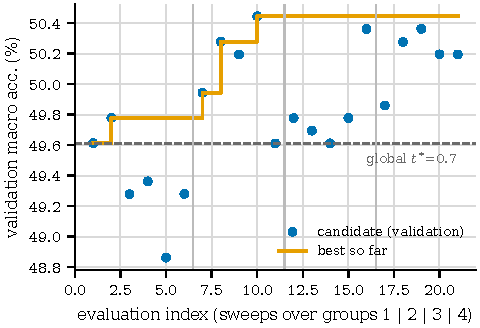
\includegraphics[width=\columnwidth]{figs/fig05b_trajectory.pdf}
\caption{Validation macro accuracy of the 21 search evaluations, in order. The step line is the best score so far; the dashed line is the global $t^*=0.7$ starting point. Most of the gain comes from the sweeps over groups 1 and 2.}
\label{fig:traj}
\end{figure}

\begin{table*}[!t]
\caption{Main comparison. Validation (1{,}199 items) and test (3{,}967 items) macro accuracy; paired differences in percentage points with 95\% bootstrap CI and two-sided $p$. Layer-wise coefficients $\hat{\mathbf t}=(0,0.75,0.7,0.7)$.}
\label{tab:main}
\centering\small
\begin{tabular}{lccccc}
\toprule
Model & Val. & Test [95\% CI] & $\Delta$ vs.\ base [95\% CI] & $p$ & $\Delta$ vs.\ $t^*$ [95\% CI] ($p$) \\
\midrule
Base (best original) & 0.4953 & 0.5025 [0.4875, 0.5174] & reference & -- & -- \\
Instruct & 0.4853 & 0.5064 [0.4909, 0.5220] & $+0.40$ [$-0.62$, $+1.41$] & 0.441 & -- \\
Global $t^*=0.7$ & 0.4961 & 0.5090 [0.4938, 0.5246] & +0.65 [$-$0.23, +1.52] & 0.149 & reference \\
Layer-wise $\hat{\mathbf t}$ & 0.5045 & 0.5129 [0.4976, 0.5280] & +1.04 [+0.20, +1.93] & 0.017 & +0.39 [$-$0.38, +1.15] (0.311) \\
\bottomrule
\end{tabular}
\end{table*}

\textbf{Hypothesis 5, first part (validation).} Table~\ref{tab:main} gives the validation and test scores. The search lifts validation from 0.4961 to 0.5045, $G_V=+0.83$ pp. As Eq.~(2) guarantees, this is non-negative; paired on the validation items it is $+0.83$ pp [$-0.58$, $+2.17$], $p=0.270$, so the gain is itself inside validation noise. This interval is computed after selection on the same items and has no nominal coverage; it is descriptive. Over the base, the validation gain of $\hat{\mathbf t}$ is $+0.92$ pp [$-0.67$, $+2.58$] ($p=0.277$).

\textbf{Second part (test).} On test, $\hat{\mathbf t}$ scores 0.5129 [0.4976, 0.5280] against 0.5090 for $t^*$: $G_T=+0.39$ pp [$-0.38$, $+1.15$], $p=0.311$. The point estimate is 47\% of the validation gain, and this is what a winner's curse predicts, but the interval contains $+0.83$ pp as well as zero, so one realization cannot separate a curse from noise. We report the comparison as not distinguishable from zero; no equivalence test was run.

\textbf{Against the best original.} $\hat{\mathbf t}$ minus the base on test is $+1.04$ pp [$+0.20$, $+1.93$], $p=0.017$. This is nominally below 0.05 but above the Bonferroni threshold 0.0083 (Fig.~\ref{fig:fig05_layerwise}), and $\hat{\mathbf t}$ was obtained by a search guided on a validation split of the same benchmarks, so we do not claim an improvement. For comparison, $t^*$ against the base is $+0.65$ pp [$-0.23$, $+1.52$] and Instruct against the base is $+0.40$ pp [$-0.62$, $+1.41$], both not distinguishable from zero. The pre-registered rule (CI above zero) would be met against the base; we do not claim an improvement for the reasons in the Statistics paragraph.

\begin{figure}[!t]
\centering
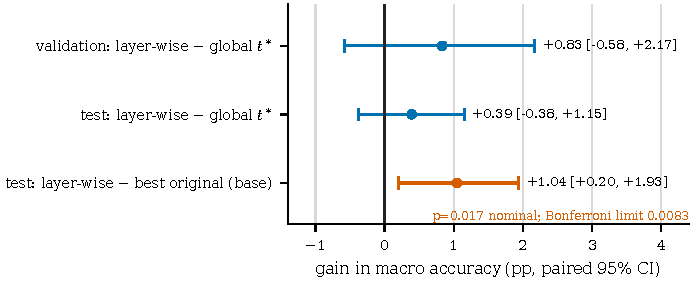
\includegraphics[width=0.85\columnwidth]{figs/fig05_layerwise.pdf}
\caption{Forest plot of three paired gains in pp with 95\% CI: validation, layers minus global $t^*$; test, layers minus global $t^*$; test, layers minus best original. The last has nominal $p=0.017$ against the Bonferroni limit 0.0083.}
\label{fig:fig05_layerwise}
\end{figure}

\textbf{Where the difference sits (descriptive).} Per-task test accuracy of $\hat{\mathbf t}$ against the base is 0.629 against 0.591 on ARC-Easy, 0.341 against 0.324 on ARC-Challenge, 0.519 against 0.525 on HellaSwag and 0.563 against 0.570 on WinoGrande, so the macro gain is carried by the two ARC tasks. No interval was computed per task, and the split by task was not pre-registered; we do not interpret it further.

\textbf{What cannot be concluded.} That layer-wise coefficients improve merging: the observed result is not distinguishable from zero over $t^*$ (no equivalence test) and a gain over the base that does not pass multiplicity correction. That the winner's curse is large: the validation gain was itself small relative to its noise. That the pattern of $\hat{\mathbf t}$ (base-like early layers, instruct-like middle layers) reflects a property of the model: the search was a single sweep with a fixed order of groups, on one set of items.

\section{Discussion and Limitations}
\textbf{Search budget.} We conjecture that the optimism is modest, but we did not measure it. The effective selection budget is about 31 configurations scored on the same 1{,}199 items: the 11 grid points that chose $t^*$ plus the 20 new configurations of the search (21 evaluations, one of which repeats $t^*$). A larger search (more groups, finer candidates, several sweeps) would score more candidates and could widen the gap between validation and test gain; we did not test this. All evaluations used bfloat16. Re-evaluating validation accuracy in fp32 at $t=0$, $0.7$ and $1$ lowered the macro accuracy by $0.67$, $0.41$ and $0.08$~pp (fp32: $0.4886$, $0.4920$, $0.4845$), a shift of the same size as the differences between coefficients, while the order of the three points did not change and WikiText-2 NLL moved by at most $0.0026$ nats at any $t$ (\texttt{results/fp32\_check\_qwen.txt}). Exact accuracy levels are therefore specific to bfloat16, and the test items were not re-evaluated in fp32. A reusable-holdout style mechanism \cite{dwork2014adaptive} or a split between search and selection would reduce the bias, at the cost of fewer items per stage.

\textbf{Scope.} One model pair at 0.5B, four commonsense and science multiple-choice benchmarks, one search run with one group order, one split seed, one hardware (Apple Silicon, bf16). Test is slightly easier than validation (about 0.50 against 0.495), so levels are not comparable across splits; only gains are. Benchmark contamination of the pretrained models is not controlled. The test CI of the gain over $t^*$ is wide (about 1.5 pp), so effects of 0.5 to 1 pp cannot be resolved with 3{,}967 items. The coordinate search keeps the best candidate so far, accepting only strict improvements, and depends on the group order; a different order might end elsewhere.

\section{Conclusion}
A one-sweep, four-group, 21-evaluation search for layer-wise interpolation coefficients of Qwen2.5-0.5B and its Instruct model raised validation accuracy by $+0.83$ pp over the global $t^*=0.7$. On 3{,}967 unseen items the gain is only $+0.39$ pp [$-0.38$, $+1.15$], not distinguishable from zero. Its $+1.04$ pp [$+0.20$, $+1.93$] gain over the best original ($p=0.017$) is nominal and fails the Bonferroni threshold 0.0083. Reports of merge improvements chosen on a validation set should give the test gain with an interval and the number of candidates scored.

\section*{Data and Code Availability}
Code, per-item caches and the search log are in the project repository at git tag \texttt{preprints-v1} (the commit that contains this manuscript and all scripts and caches); the search trajectory is \texttt{results/a5\_search.json}; scripts for the numbers and the trajectory figure written for this article are \texttt{experiments/an\_art04\_05\_tables.py} and \texttt{experiments/fig05b\_trajectory.py}. A single command regenerates all results and tables: \texttt{./run\_everything.sh}. Software: Python 3.9.6, PyTorch 2.8.0, transformers 4.57.6, NumPy 1.26.4, datasets 4.5.0. Model revisions (Hub commits, full hashes in \texttt{MANIFEST.json}): Qwen2.5-0.5B 060db6499f32, Qwen2.5-0.5B-Instruct 7ae557604adf. Split seed 0; bootstrap seed 0; the search is deterministic.

\section*{Acknowledgments}
No external funding.

\begin{thebibliography}{99}
\bibitem{yang2023adamerging} E. Yang, Z. Wang, L. Shen et al., ``AdaMerging: Adaptive model merging for multi-task learning,'' in \emph{Proc.\ ICLR}, 2024, arXiv:2310.02575.
\bibitem{huang2023lorahub} C. Huang, Q. Liu, B. Y. Lin et al., ``LoraHub: Efficient cross-task generalization via dynamic LoRA composition,'' in \emph{Proc.\ COLM}, 2024, arXiv:2307.13269.
\bibitem{akiba2024evolutionary} T. Akiba, M. Shing, Y. Tang et al., ``Evolutionary optimization of model merging recipes,'' \emph{Nat.\ Mach.\ Intell.}, 2025, arXiv:2403.13187.
\bibitem{liu2024bayesopt} D. Liu, Z. Wang, B. Wang et al., ``Checkpoint merging via Bayesian optimization in LLM pretraining,'' arXiv:2403.19390, 2024.
\bibitem{dwork2014adaptive} C. Dwork, V. Feldman, M. Hardt et al., ``Preserving statistical validity in adaptive data analysis,'' arXiv:1411.2664, 2014.
\bibitem{recht2019imagenet} B. Recht, R. Roelofs, L. Schmidt et al., ``Do ImageNet classifiers generalize to ImageNet?'' arXiv:1902.10811, 2019.
\bibitem{ilharco2022editing} G. Ilharco, M. T. Ribeiro, M. Wortsman et al., ``Editing models with task arithmetic,'' in \emph{Proc.\ ICLR}, 2023, arXiv:2212.04089.
\bibitem{wortsman2022soups} M. Wortsman, G. Ilharco, S. Y. Gadre et al., ``Model soups: Averaging weights of multiple fine-tuned models improves accuracy without increasing inference time,'' in \emph{Proc.\ ICML}, 2022, arXiv:2203.05482.
\bibitem{wortsman2022wise} M. Wortsman, G. Ilharco, J. W. Kim et al., ``Robust fine-tuning of zero-shot models,'' in \emph{Proc.\ CVPR}, 2022, arXiv:2109.01903.
\bibitem{goddard2024mergekit} C. Goddard, S. Siriwardhana, M. Ehghaghi et al., ``Arcee's MergeKit: A toolkit for merging large language models,'' arXiv:2403.13257, 2024.
\bibitem{yadav2024matters} P. Yadav, T. Vu, J. Lai et al., ``What matters for model merging at scale?'' arXiv:2410.03617, 2024.
\bibitem{yang2024survey} E. Yang, L. Shen, G. Guo et al., ``Model merging in LLMs, MLLMs, and beyond: Methods, theories, applications and opportunities,'' arXiv:2408.07666, 2024.
\bibitem{yang2024qwen25} Qwen Team, A. Yang et al., ``Qwen2.5 technical report,'' arXiv:2412.15115, 2024.
\bibitem{clark2018arc} P. Clark, I. Cowhey, O. Etzioni et al., ``Think you have solved question answering? Try ARC, the AI2 Reasoning Challenge,'' arXiv:1803.05457, 2018.
\bibitem{zellers2019hellaswag} R. Zellers, A. Holtzman, Y. Bisk et al., ``HellaSwag: Can a machine really finish your sentence?'' in \emph{Proc.\ ACL}, 2019, arXiv:1905.07830.
\bibitem{sakaguchi2019winogrande} K. Sakaguchi, R. Le Bras, C. Bhagavatula et al., ``WinoGrande: An adversarial Winograd schema challenge at scale,'' arXiv:1907.10641, 2019.
\bibitem{gao2021harness} L. Gao et al., ``EleutherAI/lm-evaluation-harness,'' Zenodo, doi:10.5281/zenodo.10256836.
\bibitem{miller2024errorbars} E. Miller, ``Adding error bars to evals: A statistical approach to language model evaluations,'' arXiv:2411.00640, 2024.
\bibitem{efron1979bootstrap} B. Efron, ``Bootstrap methods: Another look at the jackknife,'' \emph{Ann. Statist.}, 1979, doi:10.1214/aos/1176344552.
\bibitem{santos2026modelmergingfo} D. F. Santos, ``Model Merging for Capability Composition: A Technical Note,'' Zenodo, 2026, doi:10.5281/zenodo.21610555.
\bibitem{santos2026collapseresist} D. F. Santos, ``Collapse-Resistant Joint-Embedding Predictive Architectures: A Controlled Comparison of SIGReg, VICReg, and EMA,'' Zenodo, v2, 2026, doi:10.5281/zenodo.24223364.
\bibitem{santos2026knowledgedisti} D. F. Santos, ``Knowledge Distillation and Self-Distillation for Language Models,'' Zenodo, 2026, doi:10.5281/zenodo.21610100.
\bibitem{santos2026parametereffic} D. F. Santos, ``Parameter-Efficient Fine-Tuning: LoRA, QLoRA, and DoRA,'' Zenodo, 2026, doi:10.5281/zenodo.21610033.
\bibitem{santos2026mixtureofexper} D. F. Santos, ``Mixture-of-Experts Training and Sparse Upcycling,'' Zenodo, 2026, doi:10.5281/zenodo.21610062.
\bibitem{santos2026curriculumlear} D. F. Santos, ``Curriculum Learning and Data-Efficient Pretraining: A Technical Note,'' Zenodo, 2026, doi:10.5281/zenodo.21610595.
\bibitem{santos2026syntheticdatag} D. F. Santos, ``Synthetic Data Generation and Self-Improvement: A Technical Note,'' Zenodo, 2026, doi:10.5281/zenodo.21610525.
\bibitem{santos2026directpreferen} D. F. Santos, ``Direct Preference Optimization (DPO): A Technical Note,'' Zenodo, 2026, doi:10.5281/zenodo.21609911.
\end{thebibliography}

\end{document}
